\documentclass[]{standalone}
\usepackage{amsmath,amssymb}
\newcommand{\mt}[1]{\ensuremath{\mathbf{#1}}}
\newcommand{\vc}[1]{\ensuremath{\boldsymbol{#1}}}



\usepackage{pgf}
\usepackage{tikz}
\usetikzlibrary{arrows,automata,matrix}
\usepackage[latin1]{inputenc}
\begin{document}
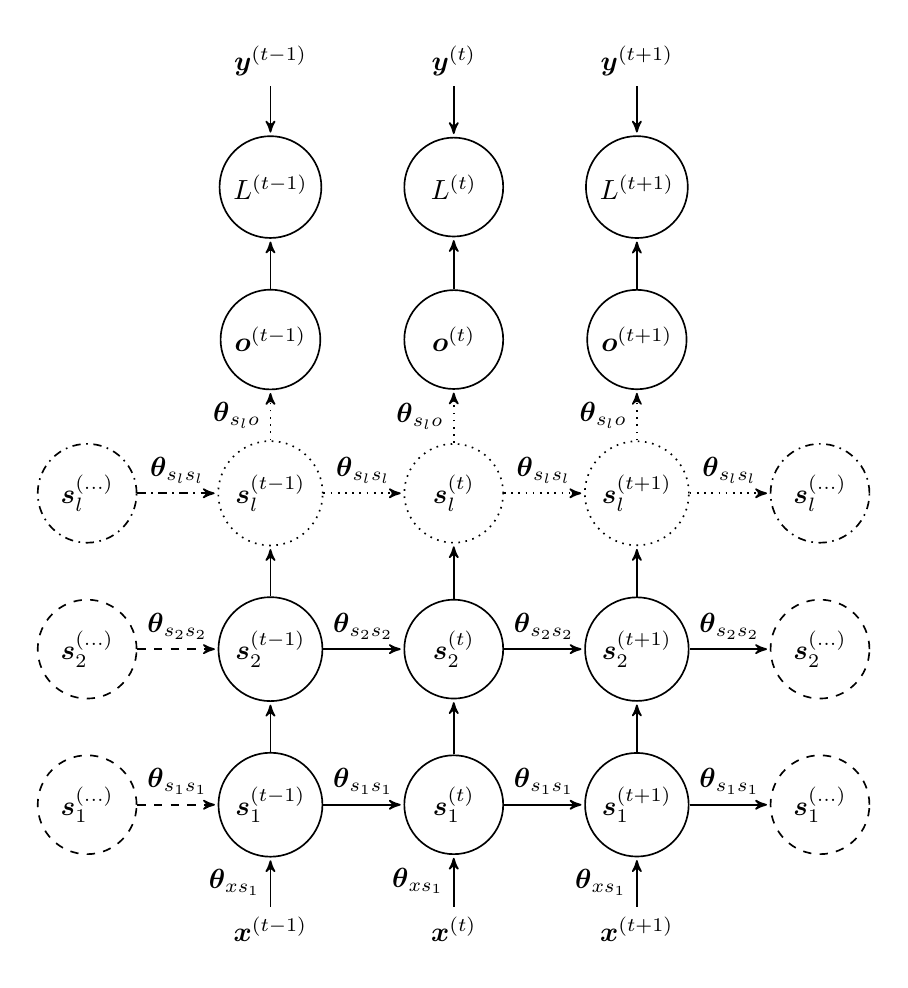
\begin{tikzpicture}[->,>=stealth'
	,shorten >=1pt
	,auto
	,node distance=2.8cm,
              semithick]
  \tikzstyle{every state}
  =[minimum size={10pt+width("$x^{(t-1)}$")}]

  \matrix (m) [matrix of nodes
  ,row sep=.25in,column sep=.4in] {
    % 3 ys
    &
    \node[](ytm1) {$\vc{y}^{(t-1)}$}; &
    \node[](yt) {$\vc{y}^{(t)}$};    &
    \node[](ytp1) {$\vc{y}^{(t+1)}$}; 
    \\
    % 3 Ls
    &
    \node[state](Ltm1) {$L^{(t-1)}$}; &
    \node[state](Lt) {$L^{(t)}$}; &
    \node[state](Ltp1) {$L^{(t+1)}$};
    \\
    % 3 os
    &
    \node[state](otm1) {$\vc{o}^{(t-1)}$}; &
    \node[state](ot) {$\vc{o}^{(t)}$}; &
    \node[state](otp1) {$\vc{o}^{(t+1)}$};
    \\
    % 5 hns
    \node[state,dashdotted](sldm) {$\vc{s}_l^{(\ldots)}$}; &
    \node[state,dotted](sltm1) {$\vc{s}_l^{(t-1)}$}; &
    \node[state,dotted](slt) {$\vc{s}_l^{(t)}$}; &
    \node[state,dotted](sltp1) {$\vc{s}_l^{(t+1)}$}; &
    \node[state,dashdotted](sldp) {$\vc{s}_l^{(\ldots)}$};
    \\
    % 5 h2s
    \node[state,dashed](s2dm) {$\vc{s}_2^{(\ldots)}$}; &
    \node[state](s2tm1) {$\vc{s}_2^{(t-1)}$}; &
    \node[state](s2t) {$\vc{s}_2^{(t)}$}; &
    \node[state](s2tp1) {$\vc{s}_2^{(t+1)}$}; &
    \node[state,dashed](s2dp) {$\vc{s}_2^{(\ldots)}$};
    \\
    % 5 h1s
    \node[state,dashed](s1dm) {$\vc{s}_1^{(\ldots)}$}; &
    \node[state](s1tm1) {$\vc{s}_1^{(t-1)}$}; &
    \node[state](s1t) {$\vc{s}_1^{(t)}$}; &
    \node[state](s1tp1) {$\vc{s}_1^{(t+1)}$}; &
    \node[state,dashed](s1dp) {$\vc{s}_1^{(\ldots)}$}; 
    \\
    % 3 xs
    &
    \node[](xtm1) {$\vc{x}^{(t-1)}$}; &
    \node[](xt) {$\vc{x}^{(t)}$};    &
    \node[](xtp1) {$\vc{x}^{(t+1)}$};
    \\
  };
  % left to right, top to bottom.
  % each layer outgoing and within itself arrows
  % minus ... 
  \path [dashdotted] (sldm)  edge  node {$\vc{\theta}_{s_ls_l}$} (sltm1);
  \path [dashed] (s2dm)  edge  node {$\vc{\theta}_{s_2s_2}$}     (s2tm1);
  \path [dashed] (s1dm)  edge  node {$\vc{\theta}_{s_1s_1}$}     (s1tm1);
  % t-1
  \path [      ] (ytm1)  edge  node {     }                 (Ltm1);
  \path [      ] (otm1)  edge  node {     }                 (Ltm1);
  \path [dotted] (sltm1) edge  node {$\vc{\theta}_{s_lo}$}     (otm1);
  \path [      ] (s2tm1) edge  node {}                      (sltm1);
  \path [      ] (s1tm1) edge  node {}                      (s2tm1);
  \path [      ] (xtm1)  edge  node {$\vc{\theta}_{xs_1}$}       (s1tm1);
  \path [dotted] (sltm1) edge  node {$\vc{\theta}_{s_ls_l}$}     (slt);
  \path [      ] (s2tm1) edge  node {$\vc{\theta}_{s_2s_2}$}     (s2t);
  \path [      ] (s1tm1) edge  node {$\vc{\theta}_{s_1s_1}$}     (s1t);
  % t
  \path [      ] (yt)    edge  node {     }                 (Lt);
  \path [      ] (ot)    edge  node {     }                 (Lt);
  \path [dotted] (slt)   edge  node {$\vc{\theta}_{s_lo}$}     (ot);
  \path [      ] (s2t)   edge  node {}                      (slt);
  \path [      ] (s1t)   edge  node {}                      (s2t);
  \path [      ] (xt)    edge  node {$\vc{\theta}_{xs_1}$}       (s1t);
  \path [dotted] (slt)   edge  node {$\vc{\theta}_{s_ls_l}$}     (sltp1);
  \path [      ] (s2t)   edge  node {$\vc{\theta}_{s_2s_2}$}     (s2tp1);
  \path [      ] (s1t)   edge  node {$\vc{\theta}_{s_1s_1}$}     (s1tp1);
  % t+1
  \path [      ] (ytp1)  edge  node {     }                 (Ltp1);
  \path [      ] (otp1)  edge  node {     }                 (Ltp1);
  \path [dotted] (sltp1) edge  node {$\vc{\theta}_{s_lo}$}     (otp1);
  \path [      ] (s2tp1) edge  node {}                      (sltp1);
  \path [      ] (s1tp1) edge  node {}                      (s2tp1);
  \path [      ] (xtp1)  edge  node {$\vc{\theta}_{xs_1}$}       (s1tp1);
  % plus ...
  \path [dotted] (sltp1) edge  node {$\vc{\theta}_{s_ls_l}$}     (sldp);
  \path [      ] (s2tp1) edge  node {$\vc{\theta}_{s_2s_2}$}     (s2dp);
  \path [      ] (s1tp1) edge  node {$\vc{\theta}_{s_1s_1}$}     (s1dp);

  
\end{tikzpicture}

\end{document}